\documentclass{scrartcl}
\usepackage{tikz}
\usetikzlibrary{positioning, arrows.meta}
\tikzset{
    arrow/.style={draw,-{Latex[length=2.5mm]}},
    block/.style={shape=rectangle,draw}
}

\begin{document}

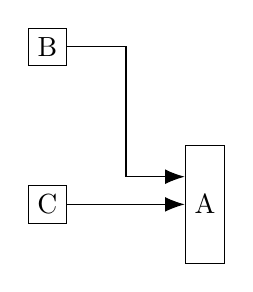
\begin{tikzpicture}
    % define distances
    \def\dist{2cm}
    \def\offset{10pt}

    % nodes
    \node [block, minimum height=1.5cm] at (0,0)            (a) {A};
    \node [block]                       at (-\dist, \dist)  (b) {B};
    \node [block, left=\dist of a.center, anchor=center]    (c) {C};

    % zwischenpunkt erstellen
    %   (mittig zwischen a und c; pos=0.75 ergibt z.B. einen zwischenpunkt 75% weg von C)
    \path (a) -- (c) coordinate [pos=0.5, above=\offset] (zp);

    % draw arrows
    \begin{scope}[arrow]
        \draw (c) -- (a);
        \draw (b) -| (zp) -- ([yshift=\offset]a.west);
    \end{scope}
\end{tikzpicture}

\end{document}

